\documentclass[12pt]{article}
\usepackage[spanish]{babel}

%%%%%%%%%%%%%%%%%%%%%%%%%%%%%%%%%%
%%%%%%%%%%%%%%%%%%%%%%%%%%%%%   %%
%%        Datos Trabajo     %%  %%
%%%%%%%%%%%%%%%%%%%%%%%%%%%%%%%%%%
\newcommand{\titulo}[0]{Actividad 2. Nombre de la actividad}
\newcommand{\materia}[0]{Estadística Básica}
\newcommand{\grupo}[0]{BI-BEBA-2002-B2-013}
\newcommand{\unidad}[0]{Unidad 2}


%%%%%%%%%%%%%%%%%%%%%%%%%%%%%%%%%%
%%%%%%%%%%%%%%%%%%%%%%%%%%%%%%%%%%
\usepackage{amssymb}
\usepackage{booktabs}
\usepackage{enumerate}
\usepackage{mathtools}
\usepackage{multicol}
\usepackage{soul}

\usepackage{geometry}
	\geometry{margin=1in}
\usepackage{graphicx}
	\graphicspath{ {assets/} }
\usepackage{hyperref}
	\hypersetup{
			pdftex,
		        pdfauthor={bench},
		        pdftitle={\titulo},
		        pdfsubject={\materia},
		        pdfkeywords={\grupo, \unidad, UnADM},
		        pdfproducer={Latex with hyperref, Ubuntu},
		        pdfcreator={pdflatex, or other tool},
			colorlinks=true,
				linkcolor=red,
				urlcolor=cyan,
				filecolor=green,
				citecolor=blue}

%%%%%%%%%%%%%%%%%%%%%%%%%%%%%%%%%%
%%%%%%%%%%%%%%%%%%%%%%%%%%%%%%%%%%

\title{
	
\includegraphics{../../../assets/logo-unadm} \\
	\ \\ Benjam\'in Rivera \\
	\bf{\titulo}\\\ \\}

\author{
	Universidad Abierta y a Distancia de México \\
	TSU en Biotecnolog\'ia \\
	\textit{Materia:} \materia \\
	\textit{Grupo:} \grupo \\
	\textit{Unidad:} \unidad \\
	\\
	\textit{Matricula:} ES202105994 }

\date{\textit{Fecha de entrega:} \today}


%%%%%%%%%%%%%%%%%%%%%%%%%%%%%
%%        Documento         %%
%%%%%%%%%%%%%%%%%%%%%%%%%%%%%%%
\begin{document}
\maketitle\newpage

	\par Las tablas de distribución de frecuencia son recursos gráficos que nos permiten apreciar la variabilidad en los datos. Técnicamente son tablas donde las abscisas se guardan las distintas freciencias que nos interesan y las ordenadas indican las agrupaciones de datos que dispongamos (hablando de las primeras de cada uno).

 \par Podemos decir que el principal objetivo de estas es el agrupar los datos para apreciar la manera en que nuestros datos se encuentran esparcidos sobre las variables de interes, y en los rangos de interes. Esto es útil para empezar a realizar hipótesis respecto a los datos con los que estemos trabajando.



\subsection*{Tabla de distribuci\'on}

\textbf{Caso}
	\begin{quote}
		Se ha realizado una encuesta en 30 hogares en la que se les pregunta el no de individuos que conviven o habitan en el domicilio habitualmente.

	Las respuestas obtenidas han sido las siguientes:
	$$4, 4, 1, 3, 5, 3, 2, 4, 1, 6, 2, 3, 4, 5, 5, 6, 2, 3, 3, 2, 2, 1, 8, 3, 5, 3, 4, 7, 2, 3$$
	\end{quote}
	\begin{figure}[h]
	\centering
		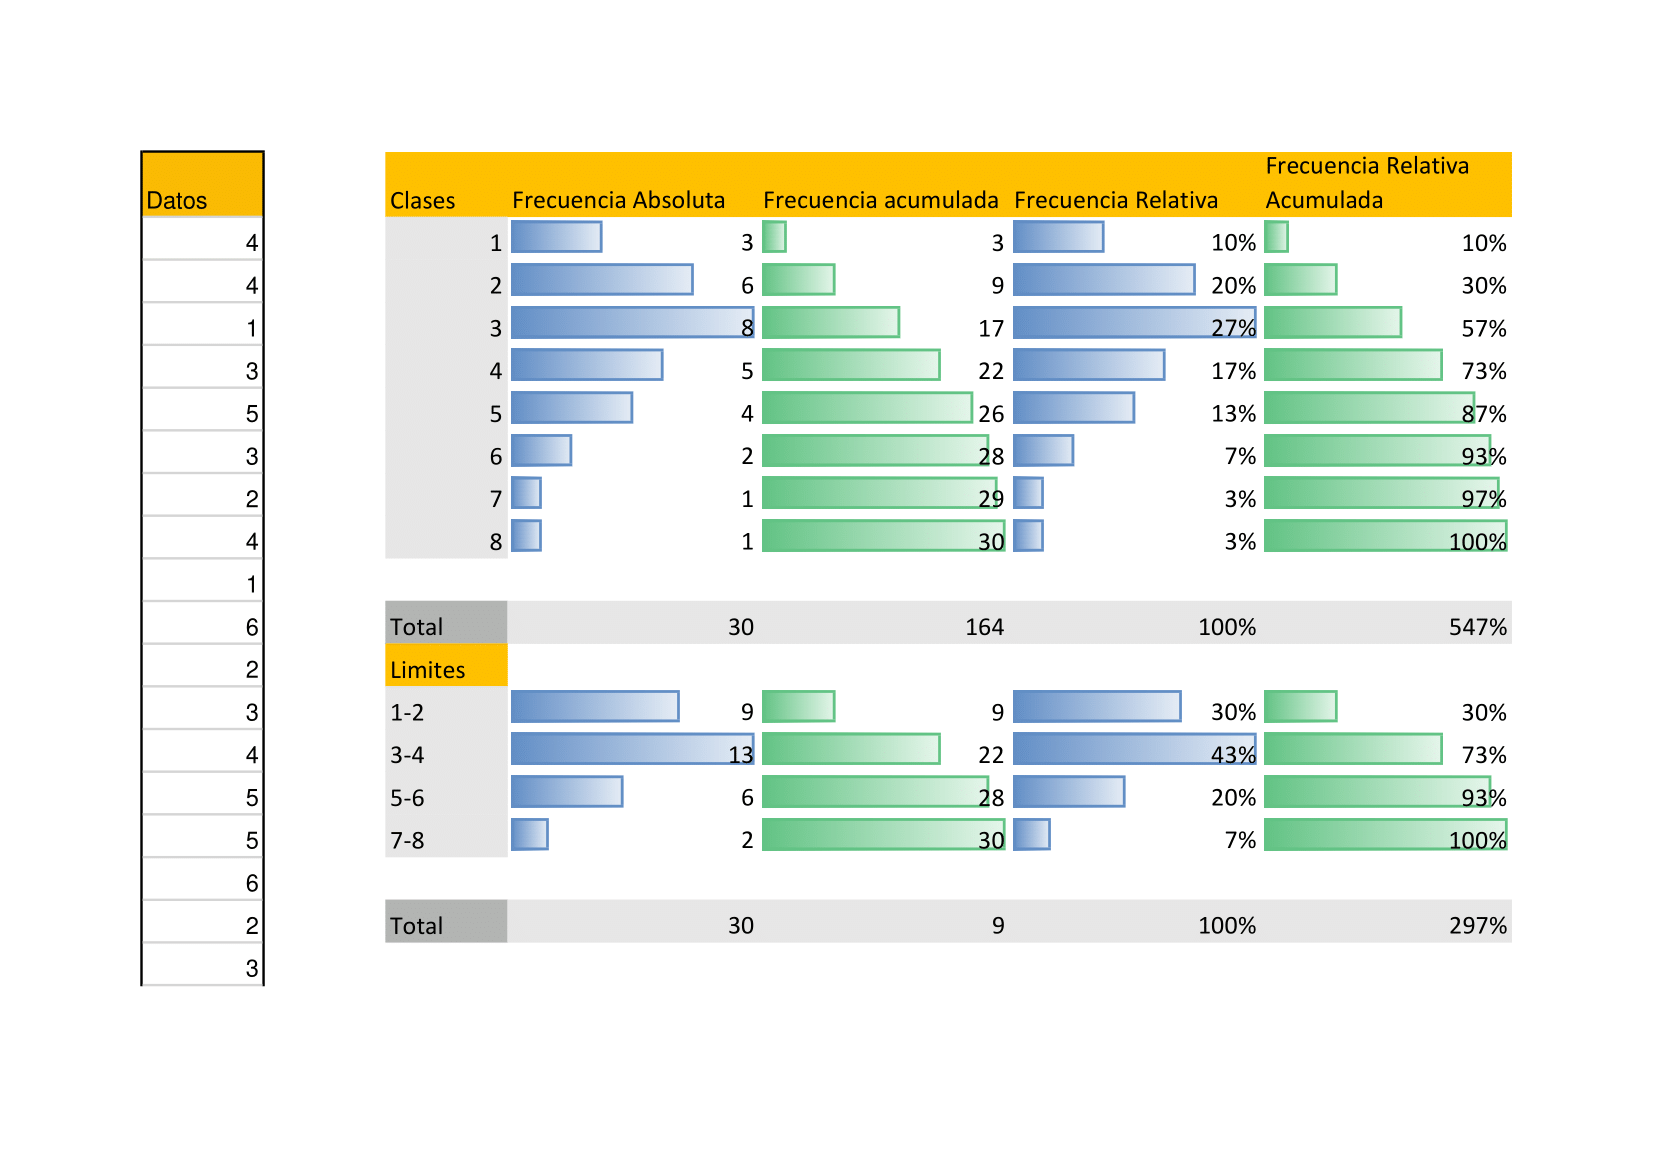
\includegraphics[width=1\textwidth]{Book1.png}
	\caption{Tablas obtenidas de excel con los datos solicitados en el ejercicio}
	\label{fig: tabla}
\end{figure}

En la Figura~\ref{fig: tabla} podemos apreciar las distribuciones tanto en las clases individuales como en clases con amplitud $2$. Para ambos conjuntos de clases se calculan las fecuencias absolutas, las relativas y las acumuladas de las dos anteriores. Los totales estan m\'as por comprobaci\'on que porque sean realmente \'utiles.

\subsubsection*{An\'alisis}

\noindent Todos los datos expresados a continuaci\'on fueron obtenidos de la Figura~\ref{fig: tabla}

\begin{itemize}
	\item \textbf{¿Qué proporción de hogares está compuesto por tres o menos personas?} 
	
	Para esto debemos fijarnos en las tres primeras clases de la primera tabla de la Figura~\ref{fig: tabla}. Dado que son las primeras $3$, entonces basta con ver la \textit{frecuencia relativa acumulada} de la clase $3$. Por lo que la proporci\'on solicitada es $57\%$
	
	\item \textbf{¿Qué proporción de individuos vive en hogares con tres o menos miembros?}
	
	Primero debemos observar que ahora queremos saber la proporci\'on de individuos, en lugar de la de hogares. Para esto primero debemos ver el total. Para esto debemos evaluar lo siguiente
	\begin{equation} T_i = \sum_{i \in C}if(i) \label{eq: Ti}\end{equation}
	donde $C$ son las clases individuales y $T_I$ es el total de individuos, que calcularemos con la suma de las multiplicaciones entre las clases $i$ y la frecuencia de estas $f(i)$. Para los datos de este ejercicio, esto nos queda que $T_i = 106$.
	Ahora debemos realizar un procedimiento similar para ver cuantos individuos estamos contando en la clase $[1,3]$. Para esto debemos resolver un caso especial de la ecuaci\'on \ref{eq: Ti}
	$$ T_3 = \sum_{i \in {1,2,3}}if(i) = 3*1 + 6*2 + 8*3 = 39$$
	Y como nos piden la proporci\'on, entonces solo falta obtener la relaci\'on entre $T_3$ y $T_i$, por lo que
	$$ \frac{T_3}{T_i} = \frac{39}{106} = 0.37 = 37\%$$ 
\end{itemize}



\subsection*{Conclusiones}

	\par Respecto a los datos que nos dieron, podemos ver que individualmente lo m\'as frecuente es que las personas vivan\footnote{en grupos de 3} con otras 2. Especificamente $27$ de cada $100$ lo hace. Por otro lado, las situaciones menos comunes es que en cada hogar vivan $7$ u $8$ personas, solo uno de cada uno por todos los hogares entrevistados.
	\par Respecto a las tablas de distribución de frecuencia. Estos elementos realmente ayduaron a que se pudiera apreciar con mayor facilidad ciertas caracter\'isticas de los datos, y me imagino que con bases de datos m\'as grandes el beneficio debe ser mayor. Aunque al final siempre terminaremos usando recursos matem\'aticos m\'as abstractos para el an\'alisis de la informaci\'on.

	



%%%%%%%%%%%%%%%%%%%%%%%%%%%%%%%%
%%         Bibliografia        %%
%%%%%%%%%%%%%%%%%%%%%%%%%%%%%%%%%%

\begin{thebibliography}{X}
	\bibitem{basico} (s. a.) (s. f.). \textit{Estadística básica. Unidad 2. Fundamentos de la estadística}. UNADM. Recuperado 3 de octubre de 2020, de \url{https://campus.unadmexico.mx/contenidos/DCSBA/TC/EBA/unidad_02/descargables/EBA_U2_Contenido.pdf}
	
	\bibitem{UV} Chorro Gascó, J. L. (s. f.). \textit{3 Distribución de frecuencias}. Universitat de València. Recuperado 7 de octubre de 2020, de \url{https://www.uv.es/webgid/Descriptiva/3_distribucin_de_frecuencias.html}
	

\end{thebibliography}

\end{document}